\documentclass[11pt, letterpaper, onecolumn]{article}
\special{papersize=8.5in,11in}

\usepackage{times}
\usepackage{amsmath}
\usepackage{fullpage}
\usepackage{epsfig}
\usepackage{subfigure}
\usepackage{setspace}

%\topmargin -0.6truein
%\textheight 9.1truein
%\textwidth 6.3truein
\sloppy

\date{}

%%%%%%%%%%%%%%%%%%%%%%%%%%%%%%%%%%%%%%%%%%%%%%%%%%%%%%%%%%%%%%%%%%%%%%
%%%%%%%%%%%%%%%%%%%%%%%%%%%%%%%%%%%%%%%%%%%%%%%%%%%%%%%%%%%%%%%%%%%%%%
%%%%%%%%%%%%%%%%%%%%%%%%%%%%%%%%%%%%%%%%%%%%%%%%%%%%%%%%%%%%%%%%%%%%%%

\title {\bf Productive Programming in Stream Computing}

\author{
  Kimberly Kuo, Rodric M. Rabbah, Saman Amarasinghe\\
  Computer Science and Artifical Intelligence Laboratory\\
  Massachusetts Institute of Technology\\
  Cambridge, MA 02139
}

\begin{document}

\maketitle

\singlespacing
\begin{abstract}
\end{abstract}

\doublespacing

%%%%%%%%%%%%%%%%%%%%%%%%%%%%%%%%%%%%%%%%%%%%%%%%%%%%%%%%%%%%%%%%%%%%%%
%%%%%%%%%%%%%%%%%%%%%%%%%%%%%%%%%%%%%%%%%%%%%%%%%%%%%%%%%%%%%%%%%%%%%%
%%%%%%%%%%%%%%%%%%%%%%%%%%%%%%%%%%%%%%%%%%%%%%%%%%%%%%%%%%%%%%%%%%%%%%

\section{Introduction}

The last  few years  have witnessed the  rebirth of  supercomputing as
computer  scientists  and engineers  realize  that current  monolithic
architectures  and conventional von~Neuman  programming styles  are at
their  limits in terms  of deliverable  end-user performance.  Thus as
architects, compiler  engineers, and application  developers look into
the  future, there  is a  concerted effort  to develop  processors and
programming   paradigms   that   can  deliver   significantly   better
performance,   and  more   so,  to   deliver  high   performance  more
productively.  This is  especially important  since the  complexity of
applications  continues to  increase, and  compilers are  more heavily
burdened with the extraction  of parallelism and the effecient mapping
of  computation  to  physical  substrate.  What's  more  is  that  the
architectures of the future  will tend toward distributed resources in
an effort  to manage the complexity of  centralized architectures with
respect to power  and wire delay. Thus, research  labs in industry and
academia alike  are investigating  ideas and methodologies  to address
the computing challenges  of the future with an  eye toward delivering
high performance and to  do so productively: $(i)$ relieve application
developers from architecture details  and allow for natural expression
of  application, $(ii)$ lessen  the burden  for heroic  compilers that
extract parallelism,  $(iii)$ develop scalable  architectures that are
powerful yet easier to verify and assemble.

The Computer Architecture Group at  MIT has for the last several years
conducted  research to  address all  of the  aformentioned objectives.
This   paper    focuses   on   the    productivitiy   of   application
developers. Specifically, the paper  will briefly describe StreamIt, a
novel language  for the prevalent application class of  stream computing. StreamIt
provides  high-level  stream   abstractions  that  improve  programmer
productivity  and  program robustness.  The  language is  architecture
independent language, and it features several characteristics (such as
parameterization  and modularity)  geared toward  large  scale program
development.  Furthermore,  this paper  will  also  describe a  unique
development  environment  that  leverages  the  language  features  to
deliver  a  toolchain for  the  rapid  verification  and debugging  of
StreamIt programs.

StreamIt represents  a program as  a hierarchical graph  of concurrent
filters  that operate  on streams  of  data and  communicate via  FIFO
queues.    The  language  exposes   the     parallelism  and
communication patterns  that are  inherent in many  streaming programs
which   include   software   radio,  real-time   encryption,   network
processing, graphics, and multimedia editing consoles.  Because of the
abundance  of parallelism  in such  applications, they  are especially
challenging  to program,  and worse,  to debug.   This is  due  to the
multitude of factors that  an application developer must consider when
implementing a streaming  program, such as for example  how to exploit
the   parallelism  on   a  target   architecture.   The   marriage  of
implementation  to a  specific processor  results in  both algorithmic
changes and  code transformations that  make porting difficult---since
the transformations depend on the architecture details.

By contrast application developers  using StreamIt focus on specifying
the functional behavior of their programs and verify correctness using
high   level  abstractions   that   result  in   clean  and   portable
implementations.   The task  of  optimizing the  code and  effeciently
mapping  it to target  processors is  left to  the compiler  which can
automate many  powerful domain specific optimizations  to deliver high
performance~\cite{streambit, linear, statespace}. This paper will not
discuss the StreamIt compiler technology; the interested reader can
visit the StreamIt web page~\cite{streamit-web}.

In  addition  to  the  language  and compiler  effort,  we  have  also
developed  a programming environment  that graphically  represents the
the hierarchical  nature of a StreamIt application.   In addition, the
StreamIt  Development  Tool  (SDT)  provides  an  elaborate  debugging
environment  that  can  interpret  and  visually  represent  streaming
computation, including  the flow of data between  streams, an intuitive
concept  of  time  for   distributed  programs,  and  a  deterministic
execution order for parallel streams.



%%%%%%%%%%%%%%%%%%%%%%%%%%%%%%%%%%%%%%%%%%%%%%%%%%%%%%%%%%%%%%%%%%%%%%
%%%%%%%%%%%%%%%%%%%%%%%%%%%%%%%%%%%%%%%%%%%%%%%%%%%%%%%%%%%%%%%%%%%%%%
%%%%%%%%%%%%%%%%%%%%%%%%%%%%%%%%%%%%%%%%%%%%%%%%%%%%%%%%%%%%%%%%%%%%%%

\section{Programming Language}
\label{sec:pl}

StreamIt~\cite{streamitcc} is an architecture-independent language for
streaming applications.   StreamIt programs are  represented as graphs
where  nodes represent  computation and  edges  represent FIFO-ordered
communication  of data  over tapes.  

The  basic programmable  unit in  StreamIt is  a filter.   Each filter
contains  a work  function which  executes atomically,  popping (i.e.,
reading)  a fixed number  of items  from the  filter's input  tape and
pushing (i.e., writing) a fixed number of items to the filter's output
tape.  A filter  can also ``peek'' at a given index  on its input tape
without  consuming  the  item;  this  makes  it  simple  to  represent
computation over a ``sliding-window''.   The push, pop, and peek rates
are  declared as  part  of  the work  function,  thereby enabling  the
compiler    to    construct    a    static    schedule    of    filter
firings~\cite{lee87static}.

%% Each filter has a distinct address space.  A filter can store two
%% types of variables: a {\it field} and a {\it local}.  Fields are
%% declared in the scope of the filter and are preserved across
%% executions, while locals are declared inside the work function and are
%% only live within a single execution.  There is also an init function
%% which runs once at the beginning of the program and is used to
%% initialize fields.
%% \begin{figure}[t]
%% \vspace{-18pt}
%% \begin{singlespace}

%% ~~
%% \begin{minipage}{0.46in}
%% {\centering
%% \psfig{figure=pipeline.eps,width=0.46in} \\
%% }
%% \end{minipage} 
%% ~
%% \begin{minipage}{1.3in}
%% {\centering
%% \psfig{figure=splitjoin.eps,width=1.3in} \\
%% }
%% \end{minipage}
%% ~
%% \begin{minipage}{1.02in}
%% {\centering
%% \psfig{figure=feedback.eps,width=1.02in} \\
%% }
%% \end{minipage}
%% ~~~~~~~~~
%% \begin{minipage}{3in}
%% \vspace{36pt}
%% \psfig{figure=iir-pipeline.eps, width=2.33in}
%% ~~~~
%% \raisebox{12pt}{\psfig{figure=iir-pipeline2.eps, width=0.46in}}
%% \end{minipage}
%% \\ ~ \\ {\protect\small (a) A pipeline. ~~(b) A splitjoin. ~~(c) A feedbackloop.}

%% \begin{minipage}{3.5in}
%% \caption{Stream structures supported by StreamIt.
%% \protect\label{fig:structures}}
%% \end{minipage}
%% \begin{minipage}{3in}
%% \caption{Example pipeline with FIR filter.\protect\label{fig:iir-pipeline}}
%% \end{minipage}
%% \vspace{3pt}
%% \hrule
%% \vspace{3pt}
%% \end{singlespace}
%% \vspace{-12pt}
%% \end{figure}

\begin{figure}[t]
\begin{center}
  \framebox{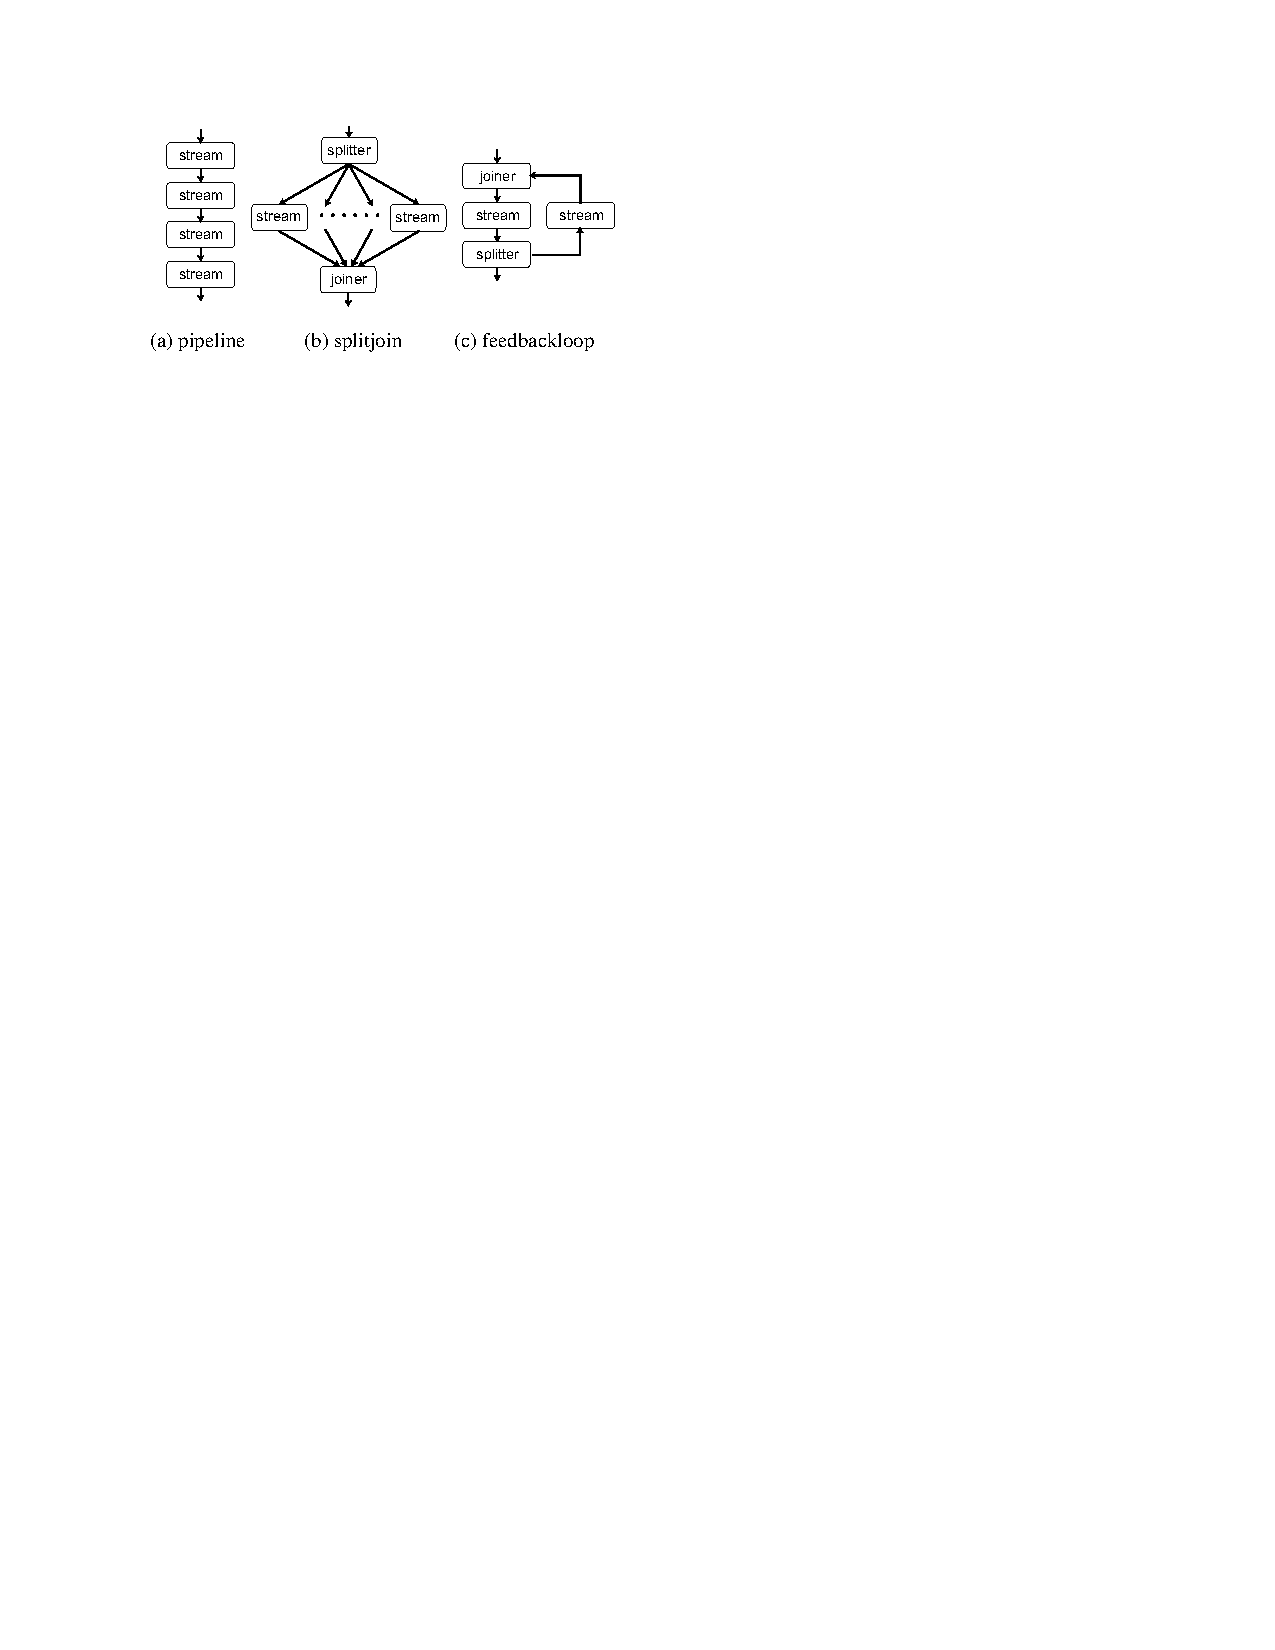
\includegraphics[scale=1, angle=0]{./constructs-eg.pdf}}
  \caption{StreamIt containers.}
  \label{fig:containers}
\end{center}
\end{figure}

\begin{figure}[t]
\begin{center}
  \framebox{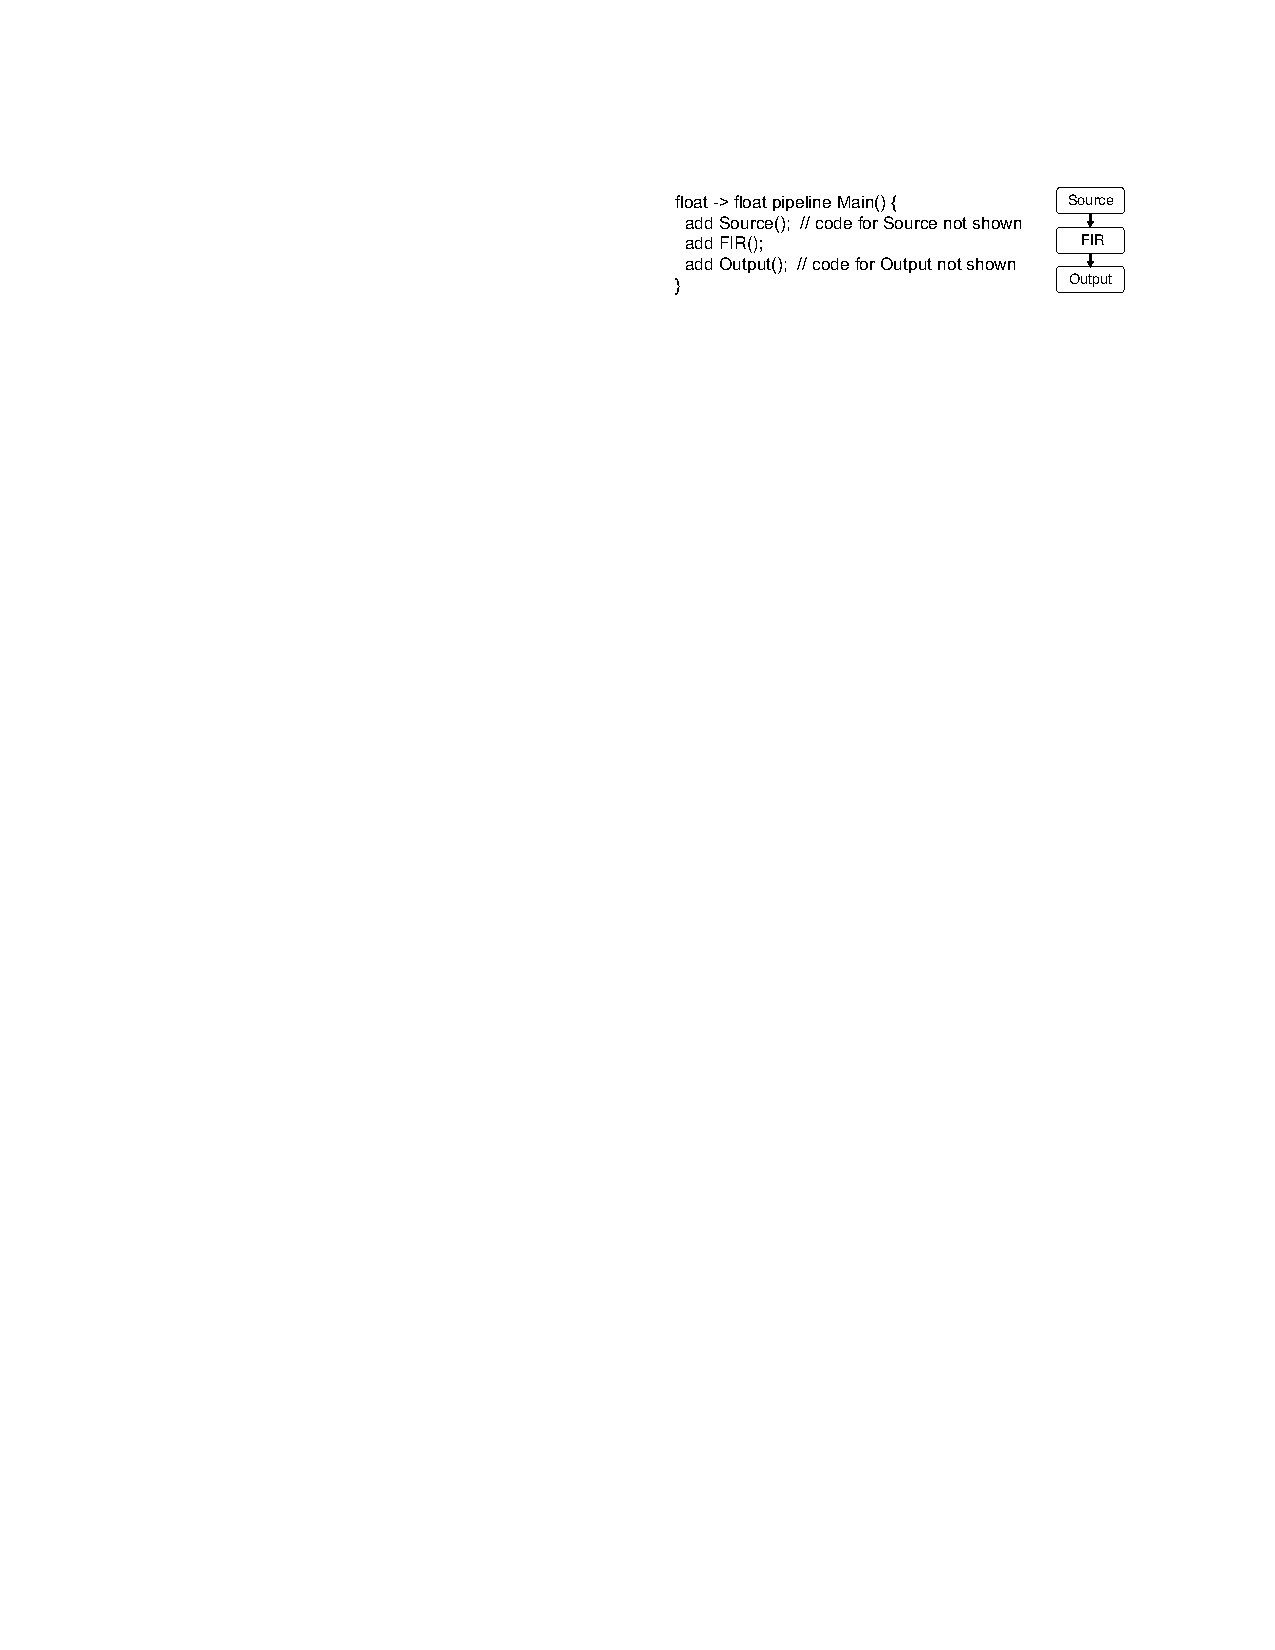
\includegraphics[scale=1, angle=0]{./pipeline-eg.pdf}}
  \caption{Example pipeline with FIR filter.}
  \label{fig:pipeline}
\end{center}
\end{figure}

StreamIt provides three  hierarchical structures for composing filters
into larger stream graphs (see Figure~\ref{fig:containers}).  The {\it
pipeline} construct  composes streams in sequence, with  the output of
one connected to the input of the next.  The {\it splitjoin} construct
distributes data to  a set of parallel streams,  which are then joined
together in a roundrobin fashion.   The {\it feedback loop} provides a
mechanism  for introducing  cycles  in  the graph.   An  example of  a
pipeline  appears  in  Figure~\ref{fig:pipeline}.  It  contains  a
single  FIR   (Finite  Impulse   Response)  filter,  which   could  be
implemented as follows:
\begin{singlespace}
\begin{verbatim}
  float->float filter  FIR(int N, float[] weights) {
    work push 1 pop 1 peek N {
      float sum = 0;
      for (int i = 0; i < N; i++) {
        sum += peek(i) * weights[i];
      }
      pop();
      push(sum);
    }
  }
\end{verbatim}
\end{singlespace}

The filter can now serve as  a module that is incorporated into stream
graphs as necessary, for example as part of an accoustic beamformer. A
filter is akin to a class in object oriented programming with the work
function  serving as  the main  method. A  filter may  also  declare a
constructor function  to initialize the filter state  before any other
method is invoked. The implementation of the work function in StreamIt
obviates  the need  for  explicit buffer  management. The  application
developer instead focuses on the  hierarchical assembly of  the stream
graph and its communication topology.

%%%%%%%%%%%%%%%%%%%%%%%%%%%%%%%%%%%%%%%%%%%%%%%%%%%%%%%%%%%%%%%%%%%%%%
%%%%%%%%%%%%%%%%%%%%%%%%%%%%%%%%%%%%%%%%%%%%%%%%%%%%%%%%%%%%%%%%%%%%%%
%%%%%%%%%%%%%%%%%%%%%%%%%%%%%%%%%%%%%%%%%%%%%%%%%%%%%%%%%%%%%%%%%%%%%%

\section{Development Environment}

The StreamIt  Development Tool (SDT)  features many aspect of  an IDE,
including a text editor and  a debugger. For example, the SDT debugger
supports line and method breakpoints, watchpoints, program suspension,
code stepping,  variable inspection and  value modification to  list a
few.

Moreover,   the  SDT   offers  features   tailored  to   the  StreamIt
language.  The  SDT  graphically  represents  StreamIt  programs,  and
preserves hierarchical information to allow an application engineer to
focus on  the aspect of  the stream program  that are of  interest. In
addition, the SDT can track the flow of data between filters, and most
importantly, it  provides a deterministic mechanism  to debug parallel
streams.

The SDT  is implemented in Java as  an Eclipse~\cite{eclispe} plug-in.
The  Eclipse universal  tools  platform is  an extansible  development
environment. We leverage the built-in user interfaces for editing and
viewing  files,  the  resource  management system,  the  documentation
infrastructure,  and the  runtime  support of  launching, running  and
debugging programs.


%%%%%%%%%%%%%%%%%%%%%%%%%%%%%%%%%%%%%%%%%%%%%%%%%%%%%%%%%%%%%%%%%%%%%%
%%%%%%%%%%%%%%%%%%%%%%%%%%%%%%%%%%%%%%%%%%%%%%%%%%%%%%%%%%%%%%%%%%%%%%

\subsection{Hierarchical Graphs}

\begin{figure}[t]
\begin{center}
  \subfigure[Collapsed pipeline.\label{fig:eg-hierarchy-collapsed}]{
    \framebox{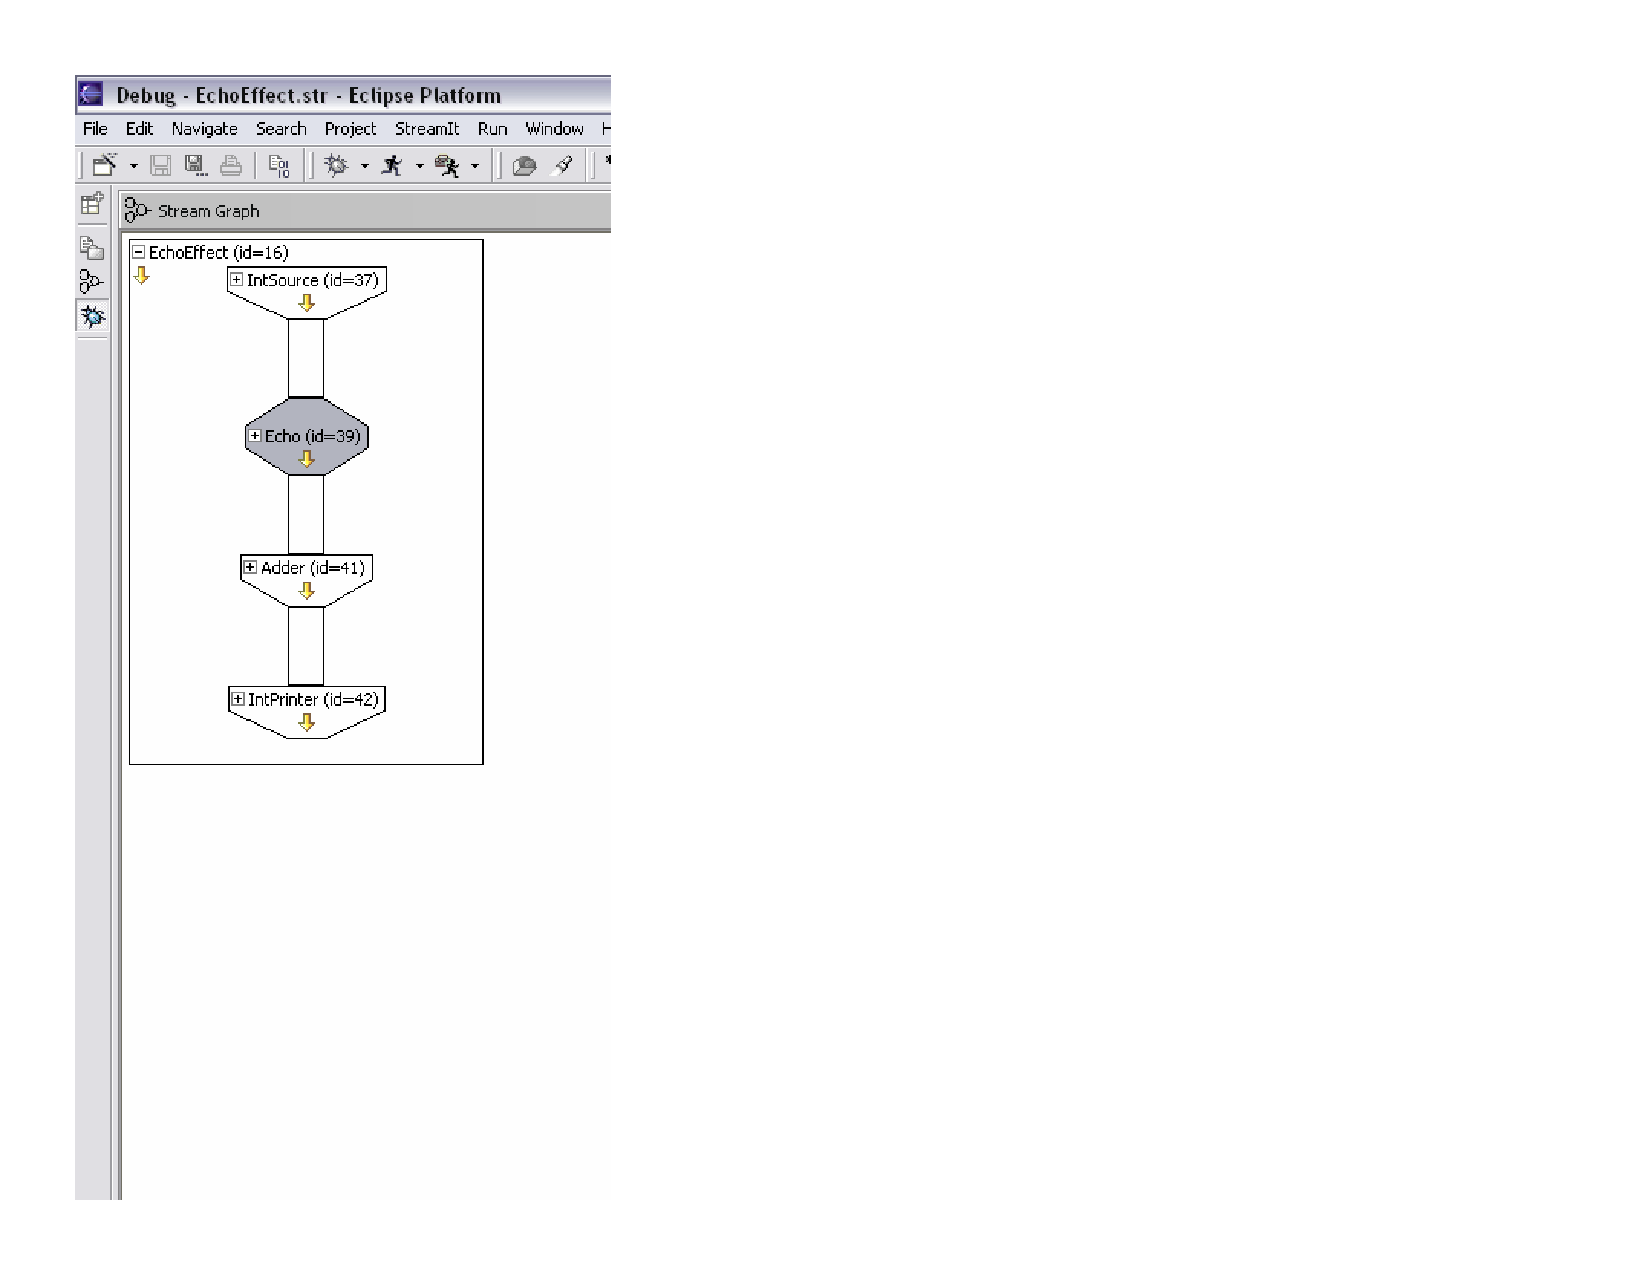
\includegraphics[scale=.4, angle=0]{./hierarchy-eg1.pdf}}
  }
  \subfigure[Expanded splitjoin.\label{fig:eg-hierarchy-expanded}]{
    \framebox{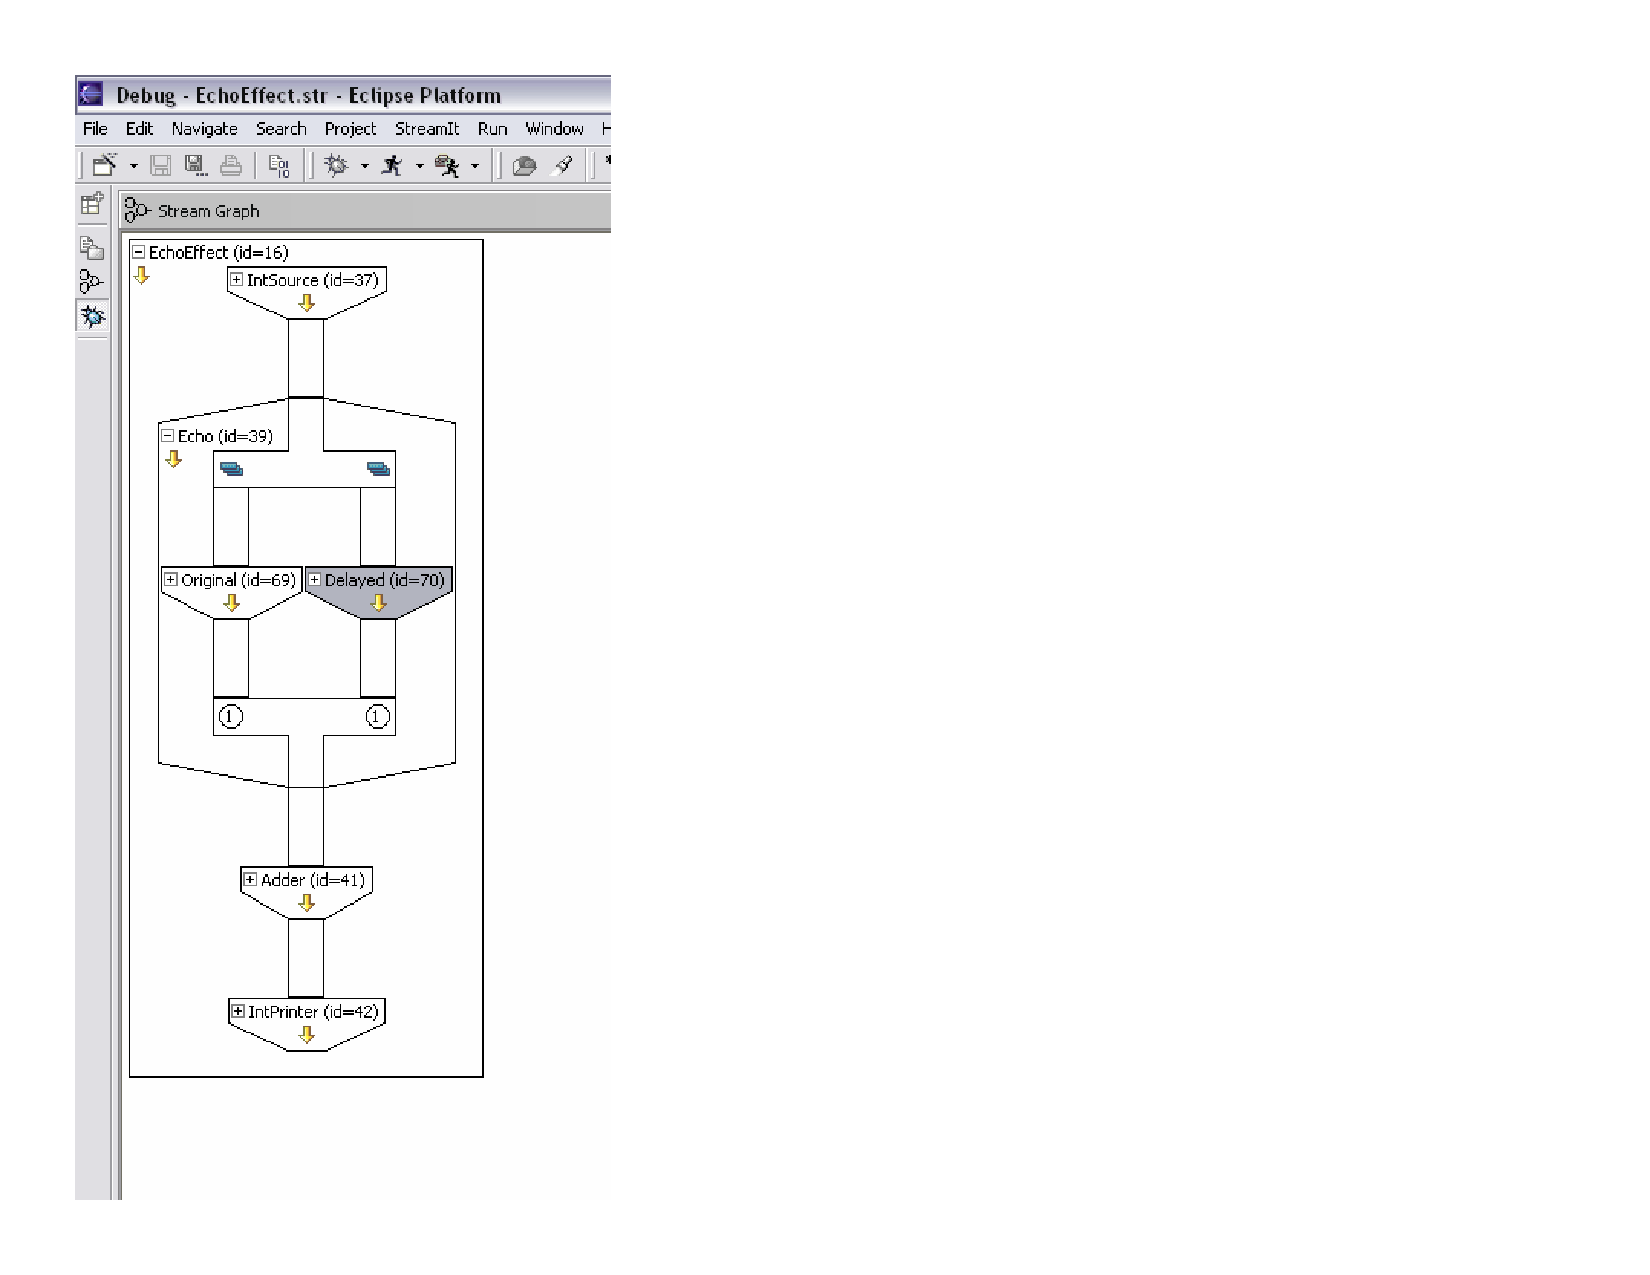
\includegraphics[scale=.4, angle=0]{./hierarchy-eg2.pdf}}
  }
  \subfigure[Example pipeline with data in transit.\label{fig:dataflow}]{
    \framebox{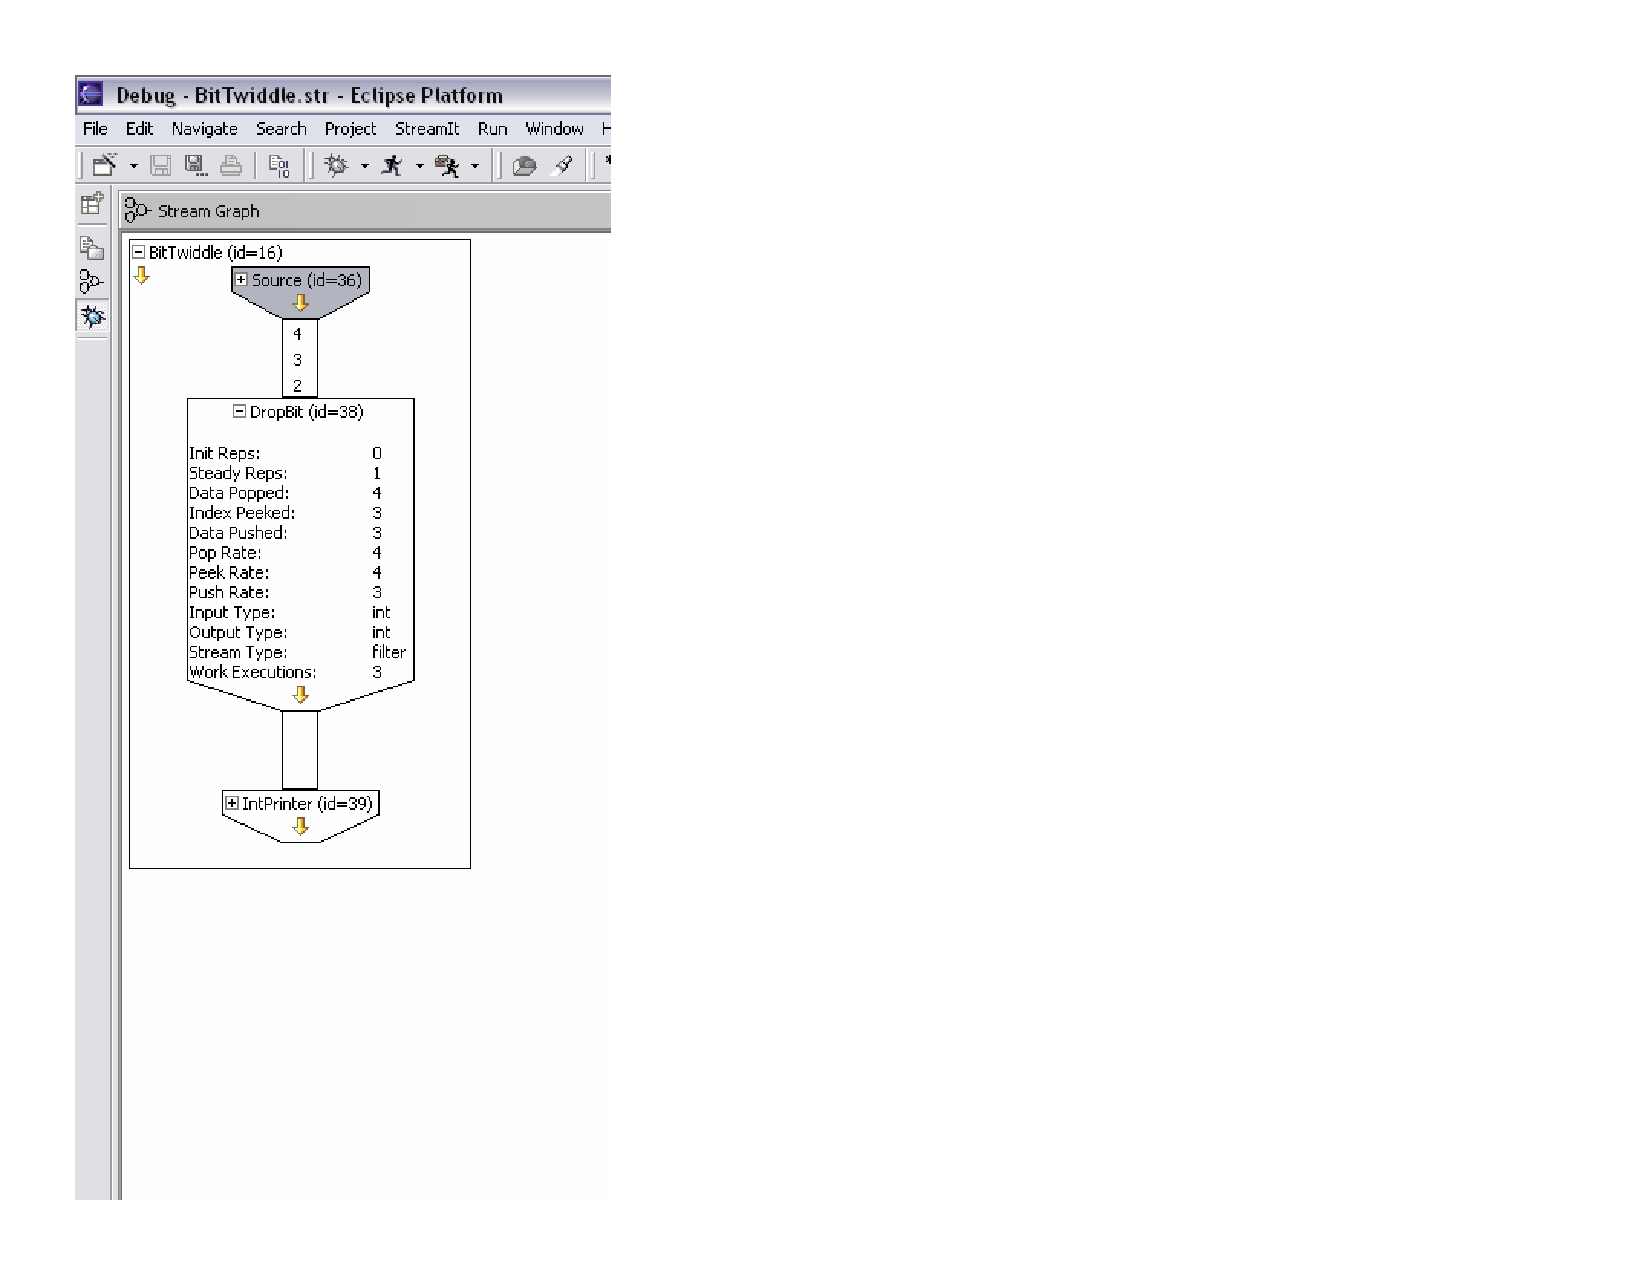
\includegraphics[scale=.4, angle=0]{./dataflow-eg.pdf}}
  }
  \caption{Hierarchical stream graph views.}
  \label{fig:hierarchy}
\end{center}
\end{figure}

As seen  in Figure~\ref{fig:eg-hierarchy},  a StreamIt program  can be
visually depicted  as a hierarchical  directed graph of  streams, with
graph nodes representing streams and graph edges representing tapes or
channels.   The   containers  are  rendered  according   to  the  code
declarations, and the visualization tools in the SDT allow the user to
selectevily collapse  and expand containers. This is  useful in large
streams  where  the  application  developers  are only  interested  in
visualizing   a  particular   subset,  for   example  to   verify  the
interconnect topology of  the graph. In Figure~\ref{fig:eg-hierarchy},
the splitjoin  is expanded whereas  the other streams in  the external
pipeline are collapsed.

%%%%%%%%%%%%%%%%%%%%%%%%%%%%%%%%%%%%%%%%%%%%%%%%%%%%%%%%%%%%%%%%%%%%%%
%%%%%%%%%%%%%%%%%%%%%%%%%%%%%%%%%%%%%%%%%%%%%%%%%%%%%%%%%%%%%%%%%%%%%%

\subsection{Data Flow}

%% \begin{figure}[t]
%% \begin{center}
%%   \framebox{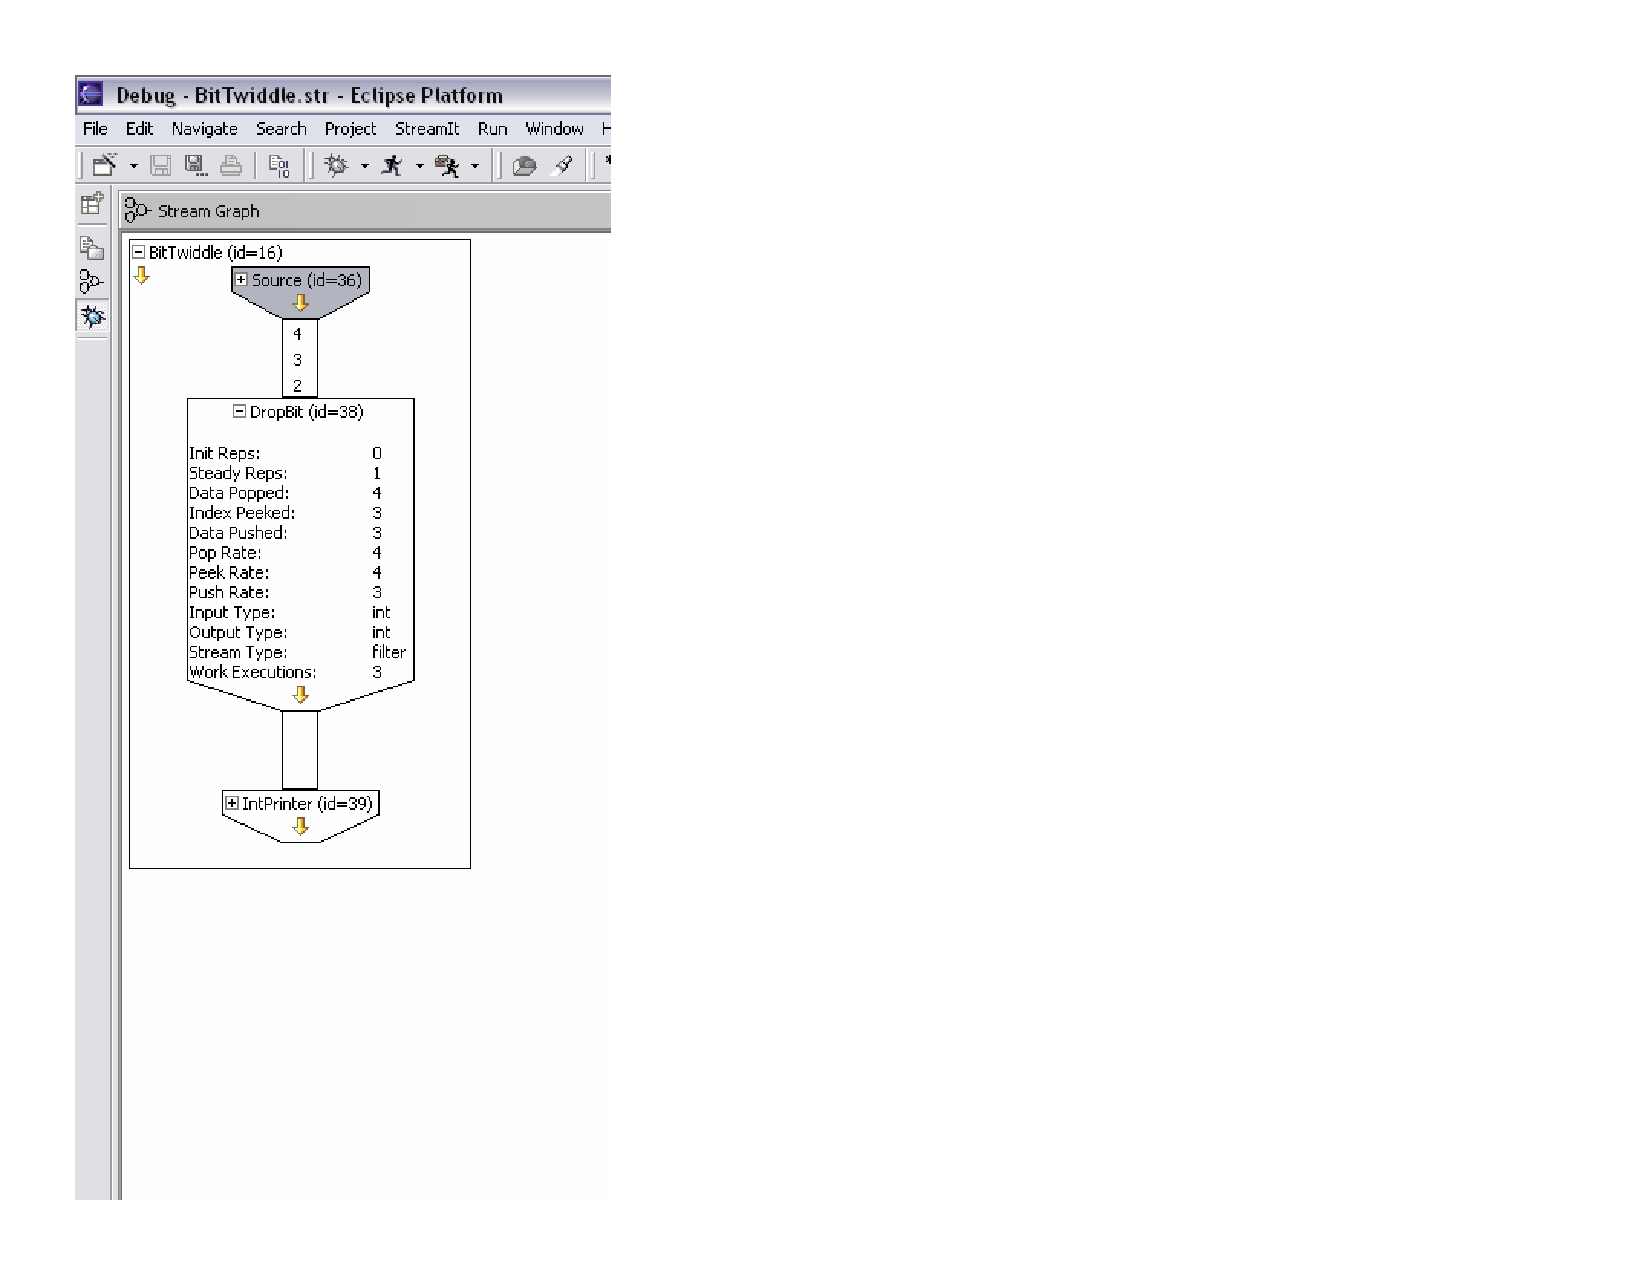
\includegraphics[scale=1, angle=0]{./dataflow-eg.pdf}}
%%   \caption{Example pipeline with data in transit.}
%%   \label{fig:dataflow}
%% \end{center}
%% \end{figure}

An important distinguishing characterisitic  of the SDT is its ability
to track  the flow  of data between  streams.  This is  illustrated in
Figure~\ref{fig:dataflow} which shows the data that is live between
two filters.  The  SDT allows the user to  highlight and automatically
track  data items  as they  propagate between  streams.  The  SDT also
allows the user  to modify values on a tape,  much like a conventional
debugger allows users to modify variables and registers.

The flow of data is especially helpfull in splitjoins where sequential
data streams are distributed to parallel streams, and parallel streams
assembled into a single stream. The visulalizations allows the user to
readily  verify  that  splitters  and joiners  implement  the  desired
functionality.  Also,  the   visualization  allows  users  to  quickly
pinpoint unexpected outputs (e.g., a filter pushing NaN's).

%%%%%%%%%%%%%%%%%%%%%%%%%%%%%%%%%%%%%%%%%%%%%%%%%%%%%%%%%%%%%%%%%%%%%%
%%%%%%%%%%%%%%%%%%%%%%%%%%%%%%%%%%%%%%%%%%%%%%%%%%%%%%%%%%%%%%%%%%%%%%

\subsection{Debugging Parallel Streams}

Perhaps  the most  important feature  of the  SDT is  its  support for
debugging parallel  streams. In StreamIt,  the streams in  a splitjoin
are  independent,  and can  fire  when  their  corresponding data  are
queued. Unlike threads in parallel programs, there is a unique program
counter,  and a  deterministic schedule  that  the SDT  can follow  to
execute parallel streams.  Furthermore,  by tracking the flow of data,
StreamIt provides a natural way  to reason about time in a distributed
system  thereby greatly  simplifying  the task  of debugging  parallel
streaming programs.

%%%%%%%%%%%%%%%%%%%%%%%%%%%%%%%%%%%%%%%%%%%%%%%%%%%%%%%%%%%%%%%%%%%%%%
%%%%%%%%%%%%%%%%%%%%%%%%%%%%%%%%%%%%%%%%%%%%%%%%%%%%%%%%%%%%%%%%%%%%%%
%%%%%%%%%%%%%%%%%%%%%%%%%%%%%%%%%%%%%%%%%%%%%%%%%%%%%%%%%%%%%%%%%%%%%%

\section{Productivity Study}

We designed and carried out a  user study to assess the extent the SDT
helps in debugging StreamIt programs.  The goals were two fold. First,
we aimed to identify difficulties in using the SDT and toward this end
we used questionnaires and  automatic action logging.  The second goal
was to gather data to support  the hypothesis that the SDT can improve
a programmer's ability to debug StreamIt applications.

We provided  participants with a  set of ``buggy''  StreamIt programs,
along with verbal descriptions of the programs.  The participants were
asked to find and fix the  errors and to record their experience using
various forms  and questionaries.  The participants  were divided into
different  groups,  some of  which  used  the  SDT and  its  graphical
debugging features  whereas others did not.  Our  results and analysis
are repored  in the  following section, following  the details  of the
study.

%%%%%%%%%%%%%%%%%%%%%%%%%%%%%%%%%%%%%%%%%%%%%%%%%%%%%%%%%%%%%%%%%%%%%%
%%%%%%%%%%%%%%%%%%%%%%%%%%%%%%%%%%%%%%%%%%%%%%%%%%%%%%%%%%%%%%%%%%%%%%

\subsection{Target Population}

We solicited participants for the  user study by advertising it to MIT
students population majoring in  computer science. We favored students
who specialize in  communications, signal processing, computer systems
and  architecture,  and  who  are experienced  in  popular  imperative
languages  (e.g.,  C,  C++,  Java).   The  nature  of  study  was  not
explicitly  divulged  in  our  solicitation; this  served  to  prevent
potential  users from  learning about  StreamIt and  becoming familiar
with the SDT  prior to the study. The particpants  were awared a small
monetary gift upon completion of the study.

%%%%%%%%%%%%%%%%%%%%%%%%%%%%%%%%%%%%%%%%%%%%%%%%%%%%%%%%%%%%%%%%%%%%%%
%%%%%%%%%%%%%%%%%%%%%%%%%%%%%%%%%%%%%%%%%%%%%%%%%%%%%%%%%%%%%%%%%%%%%%

\subsection{Methodology}

Each participant in the user study was presented with a  set of
documents that described the tasks of the study and which served to
record information from the particpants during the study. The
documents were:
\begin{enumerate}
\item Pre-Study  Questionnaire: This  document was designed  to gather
information  on  the participant's  programming  background and  skill
level. Questions such  as year in school, major,  degree being sought,
area  of computer  science concentration,  relevant  classes, language
proficiency,  application development  experience,  and background  in
DSP, IDE, and the SDT are asked.
\item  StreamIt  Language  Tutorial:  This  written  presentation  was
intended to give  a cursory introduction to the  StreamIt language. It
described  and illustrated the  syntax and  semantics of  the StreamIt
language. Furthermore,  example toy applications and tips  on the most
common  mistakes new  StreamIt  programmers are  likely  to make  were
included.
\item SDT  Tutorial: Another  written presentation, this  document was
aimed at  informing users  of the essential  features of the  SDT. The
first part of the tutorial described the functionality of the StreamIt
editor  and  debugger.  The  second  part of  the  document  contained
step-by-step instructions on  how to compile, run, and  debug a sample
application.
\item  User  Tasks:  This  document  instructed users  to  debug  nine
StreamIt applications in  a specific order. Each of  the nine programs
contained one  or more bugs.  As  the users moved from  program to the
next,  they  were asked  to  record their  start  and  end times,  the
debugging methods they used  (e.g., code inspection, print statements,
graphical debugger),  and a short  diagnosis of the program  bugs they
uncovered.
\item Description of Applications  and Code: This document contained a
description  of  each  application  (numbered  1 through  9),  a  code
listing, a sample buggy output, and a sample correct output. The
applications are summarized in Table~\ref{tab:applications}.
\item Post-Study  Questionnaire: This document was  designed to gather
data   on  the   participant's   experience.  Furthermore,   questions
pertaining to the  perceived difficulty of each problem  and a general
description of  how the user  debugged each application are  asked, in
addition to questions concerning  bugs, satisfaction, ability to learn
and  remember,  speed  after  learning, ease  of  use,  functionality,
comments, and improvements related to the SDT.
\end{enumerate}

In  order  to control  against  the  SDT's  effect on  a  programmer's
debugging  ability and  ensure internal  validity, users  were grouped
into four categories,  which were based on which  applications were to
be     debugged     with      and     without     the     SDT     (see
Table~\ref{tab:apps-groups}).    All  users   were   asked  to   debug
application 1 without the SDT and application 2 with the SDT to assess
starting ability and create a baseline reference for later comparison.
Moreover, these  two ``control'' application were  designed to bolster
the user's confidence.  Then, half of the users (group A) were told to
debug applications 3,  4, and 5 with  the SDT and 6, 7,  and 8 without
the SDT. Meanwhile, the other half  (group B) were told to debug 3, 4,
and 5 without the  SDT and 6, 7, and 8 with  the SDT to avoid ordering
effects.  Due to this grouping  structure, applications 3 and 6, 4 and
7,  and 5  and 8  were written  to be  of comparable  difficulty.  For
application 9,  half of  group A (A1)  and half  of group B  (B1) were
asked to debug  with the SDT, while the other halves  (A2 and B2) were
asked to debug without the SDT.  Cross-sectioning the groups was aimed
at ensuring external validity.

The study was divided into three sessions over a three-day period.  We
estimated that each session would  last for two hours (with 45 minutes
spent  on  the  tutorials  and  the  rest of  the  time  dedicated  to
debugging), but  in reality  the sessions spanned  an average  of four
hours.  Many users  were either unable or did not  have enough time to
debug certain  applications.  Participants were asked  to complete the
set of documents at their own pace.  Upon completion of the study, the
participants were  individually interviewed  and received a  \$40 gift
certificate.  During the study, users were encouraged to ask questions
although particulars  relating to  the problems and  the SDT  were not
revealed.

%%%%%%%%%%%%%%%%%%%%%%%%%%%%%%%%%%%%%%%%%%%%%%%%%%%%%%%%%%%%%%%%%%%%%%
%%%%%%%%%%%%%%%%%%%%%%%%%%%%%%%%%%%%%%%%%%%%%%%%%%%%%%%%%%%%%%%%%%%%%%

\subsection{Results and Analysis}

Eventhough 25  users were  scheduled  to participate  (5 people  for
sessions 1 and  2 and 15 people for  session 3), cancellations reduced
the participation to 20 users  and led to uneven groupings. There were
6 people in A1, 5 in A2, 4 in B1, and 5 in B2. Of the 20 participants,
there were 4 juniors, 2 seniors,  8 masters, and 6 Ph.D. students, all
majoring in Electrical Engineering and Computer Science. Although none
had used the SDT in the past, 6 users had experience with DSP.

\begin{figure}[t]
\begin{center}
  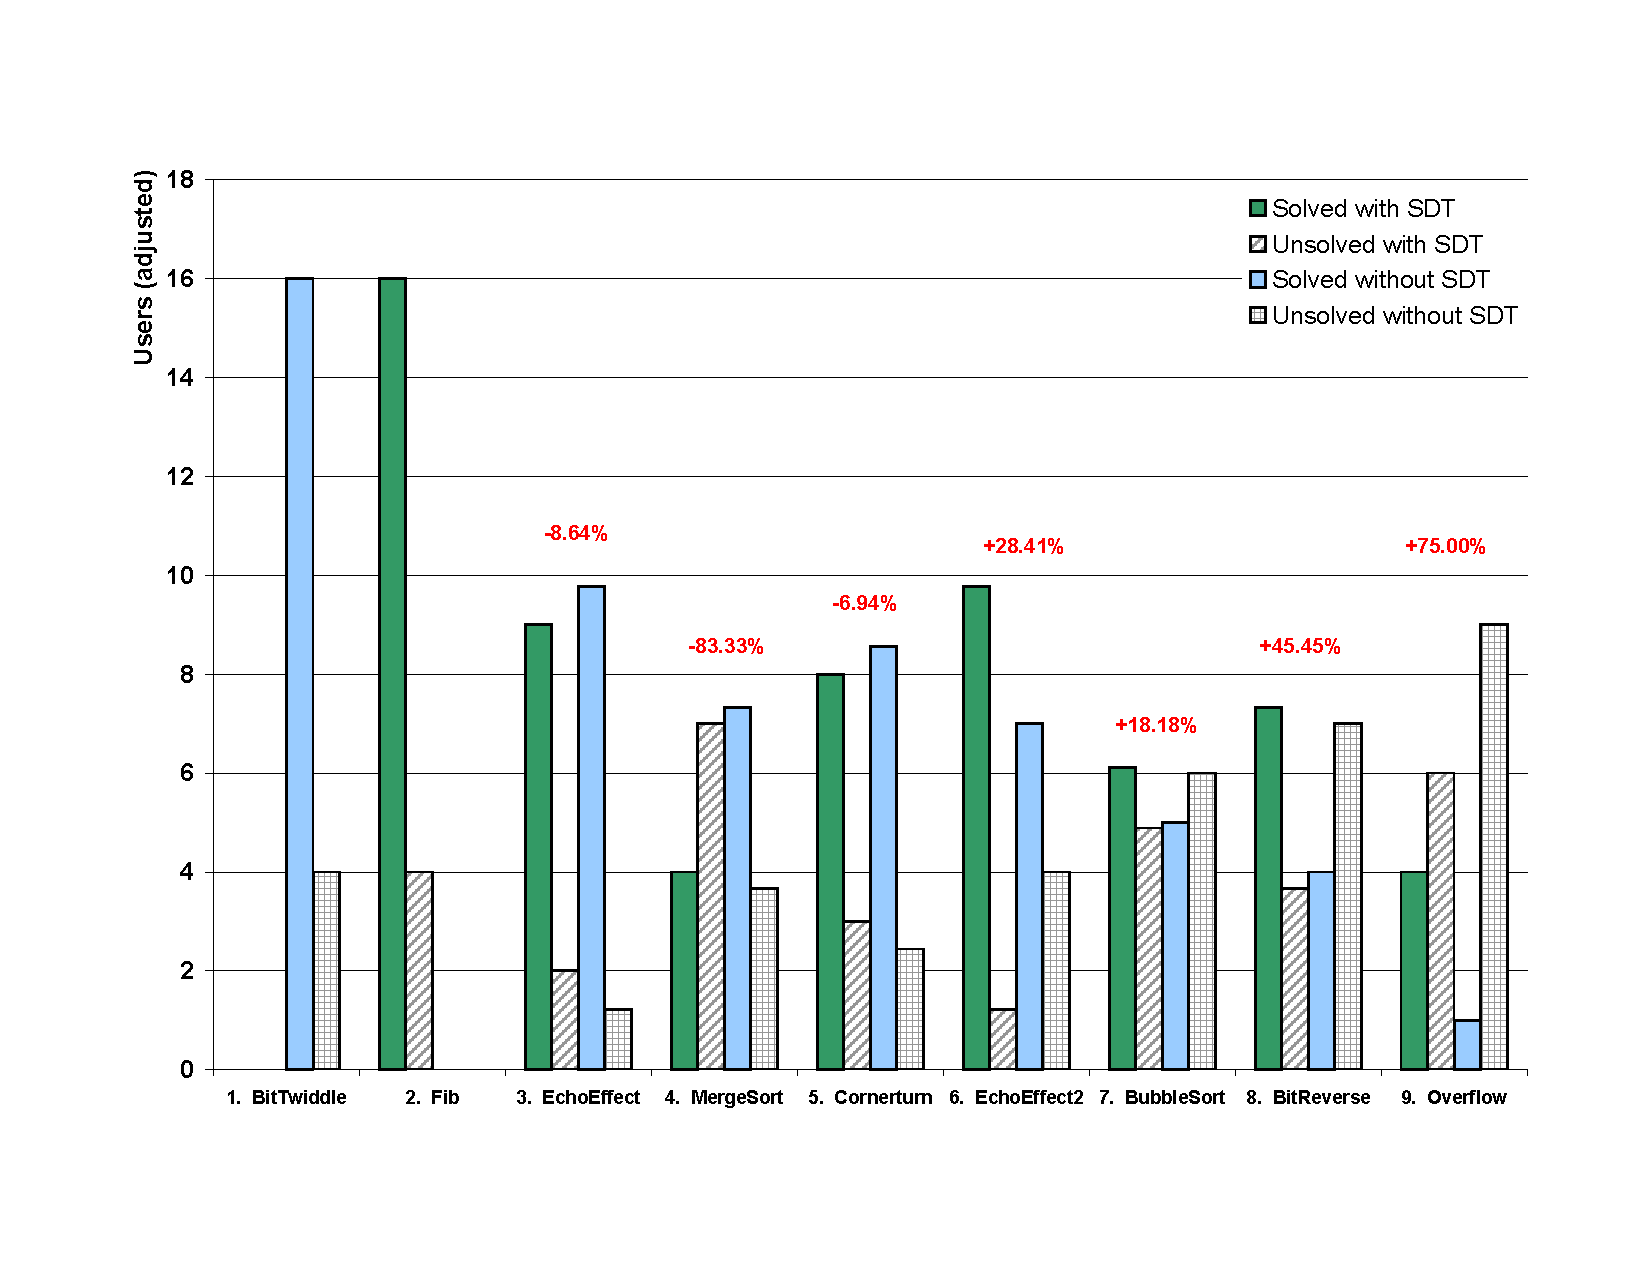
\includegraphics[scale=.5, angle=0]{./users-results.pdf}
  \caption{Summary of results.}
  \label{fig:solutions}
\end{center}
\end{figure}

Figure~\ref{fig:solutions} summarizes the study in terms of the number
of solutions  reported for each of  the applications in  the study. In
the figure,  the bars  labeled ``solved with  the SDT''  represent the
number   of  participants  that   fully  debugged   the  corresponding
applications  using  the SDT.  Similarly,  the  bars labeled  ``solved
without  the SDT''  represent the  number of  participants  that fully
debugged  the corresponding applications  without using  the graphical
debugger. The bars that  are labeled ``unsolved'' represent the number
of participants  whose applications  remained buggy. For  example, for
the application \texttt{EchoEffect} there were two users who were
allowed to used the SDT and were unable to debug the code
properly. There was also one other participant who did not debug
\texttt{EchoEffect} although this user was not allowed to use the SDT.

Because the groupings are  uneven as previously mentioned, the numbers
seen in  the figure are weighted  depending on which  group is lacking
users. The  percentage above each quadruple of  columns represents the
percentage increase  or decrease in  debugging each application  due to
the  SDT.   For  example,  the   SDT  did  not  particularly  help  in
applications  3,  4,  and 5,  but  does  help  for  all of  the  other
applications.   On  average, 1.56  fewer  participants fully  debugged
applications  3, 4,  and 5  when using  the SDT,  and 2.56  more users
solved applications  6, 7,  8, and  9 when using  the SDT.

\begin{figure}[t]
\begin{center}
  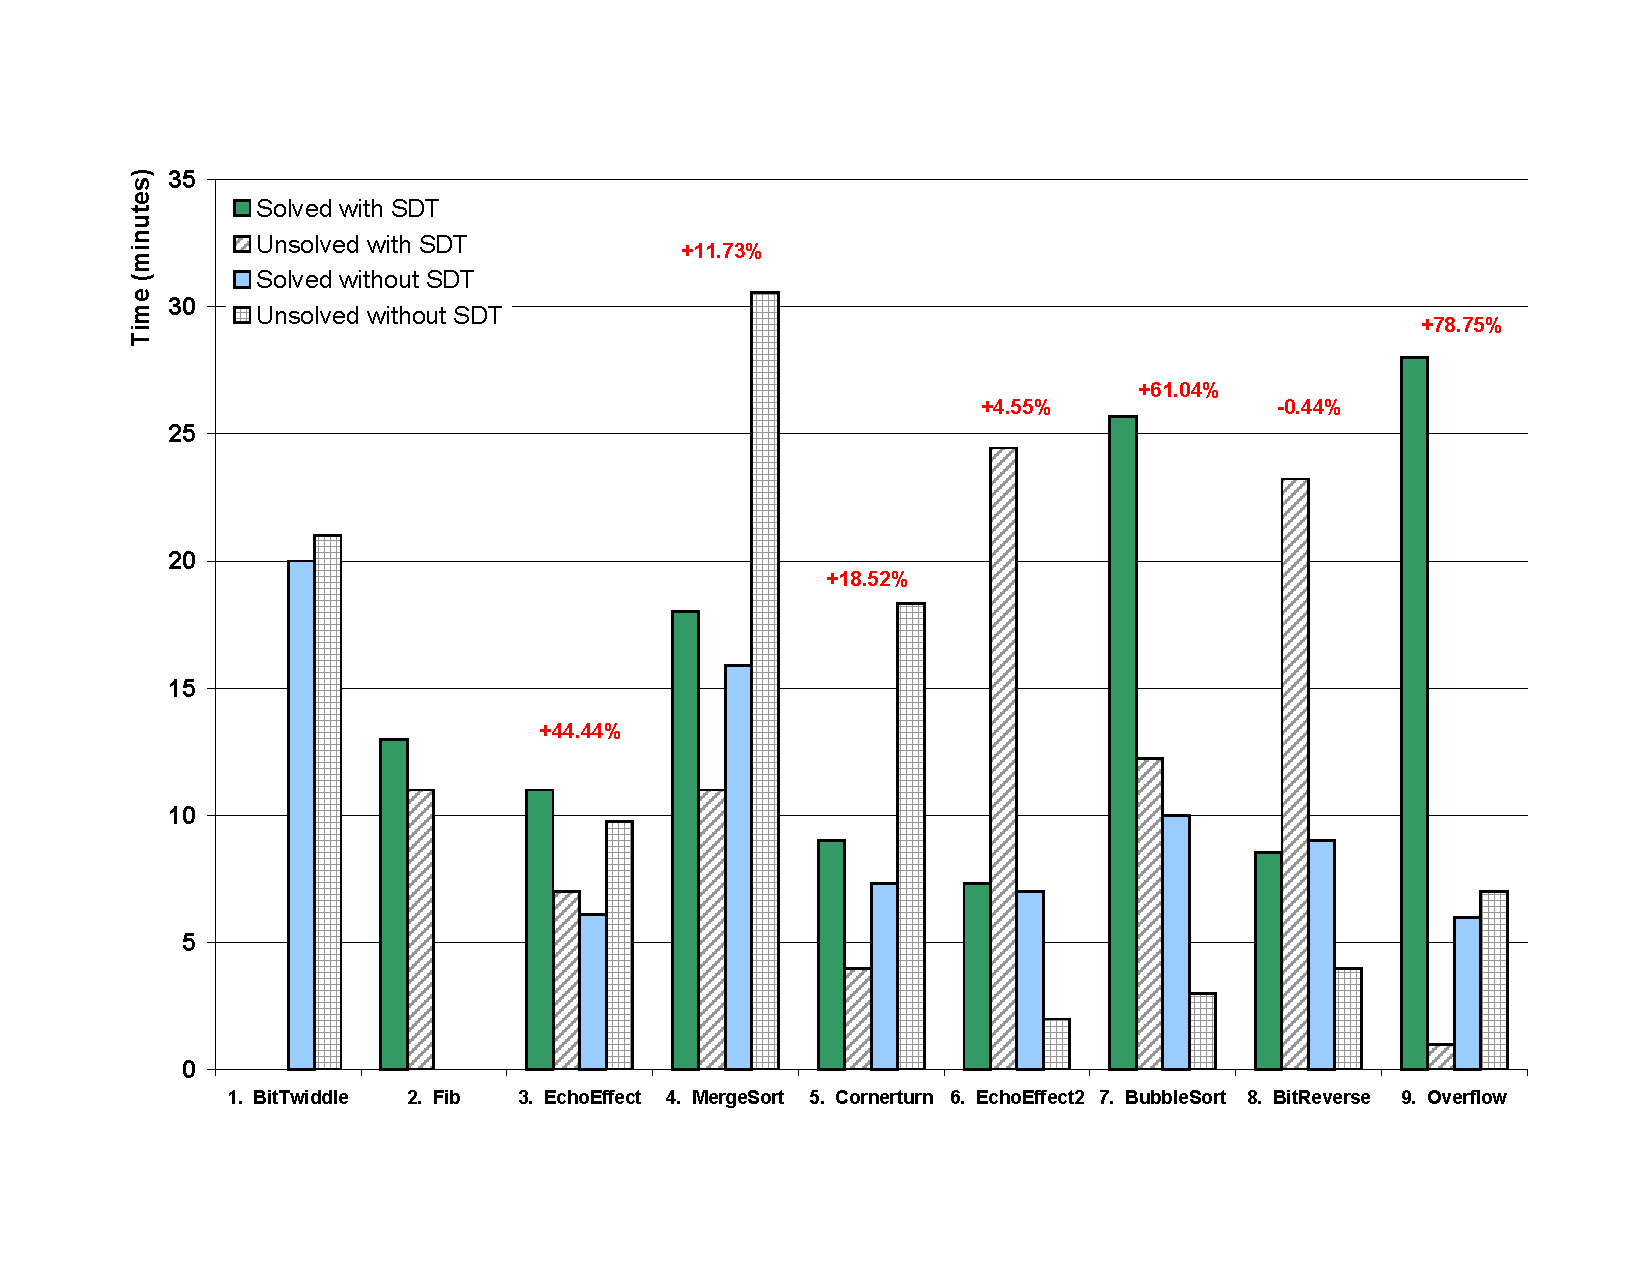
\includegraphics[scale=.5, angle=0]{./times-results.pdf}
  \caption{Summary of results.}
  \label{fig:times}
\end{center}
\end{figure}

Figure~\ref{fig:times} compares the  average time spent debugging each
application. The  percentage above each set of  columns represents the
percentage improvement or deficiency in  time caused by using the SDT.
On  average,   users  took  7.78  (36.48\%)  more   minutes  to  solve
applications 3, 4, 5, 6, 7, and 9 when using the graphical featuers of
the  debugger,   compared  to  participants   using  more  traditional
debugging means. Furthermore, participants who were allowed to use the
SDT and its graphical features  spent an avearge of 16.96 more minutes
debugging applications  6, 7,  and 8, compared  to an average  of 10.67
minutes invested by  the participants who could not  use the graphical
debugger. In  both cases  the participants did  not fully  debug their
respective applications.

Summarizing the results, we found  that more participants were able to
successfully  debug their  applications  when using  the  SDT and  its
graphical features.  However, we also observed that  the SDT increased
the  ``time to  solution'' as  users had  to navigate  through  a user
interface  they were  not familiar  with. Interestingly,  we  can also
observe  that  the  SDT   may  have  mitigated  user  frustration.  As
previously mentioned, because users  generally took much more than the
two  hours  allotted  to   complete  the  study,  users  often  became
frustrated  or rushed  with the  later  applications. Correspondingly,
this  might have  caused  users to  spend  less time  and solve  fewer
applications  as users  progressed  through the  study. Although  this
pattern is true for participants who did not use the SDT, the opposite
occurs  for participants who  used the  SDT: Eventhough  32.97\% fewer
users  were able  to solve  applications 3,  4, and  5 when  using the
graphical debugger, 41.76\% more users were able to solve applications
6, 7,  8, and 9 using  the SDT. Furthermore, users  spent 83.35\% more
time when  unable to  solve applications  6, 7, and  8 when  using the
graphical debugger.  These results suggest  that users are  willing to
spend more time and work on more problems when using a tool that they
felt more certain would lead them to a solution.

%%%%%%%%%%%%%%%%%%%%%%%%%%%%%%%%%%%%%%%%%%%%%%%%%%%%%%%%%%%%%%%%%%%%%%
%%%%%%%%%%%%%%%%%%%%%%%%%%%%%%%%%%%%%%%%%%%%%%%%%%%%%%%%%%%%%%%%%%%%%%

\subsection{User Feedback}

Qualitative data  obtained from the post-study  questionnaires was
quite helpfull toward  finding  new   feature  ideas  and  problems  with
functionality, performance, reliability, and usability.

Summarizing  the most  notable  feedback, users  largely commented  on
their difficulties using Eclipse and navigating the StreamIt code. Ten
participants commented that Eclipse was difficult to get familiar with
in the  time alloted, and there  was an over abundance  of windows and
options  to  choose  from,  and therefore  finding  vital  information
immediately  was  slow.   Five   participants  noted  that  they  were
uncomfortable  or  unaccustomed  to  thinking  in  terms  filters  and
streams, while an equal number  also found it overwhelming to remember
some of the language syntax and concepts.

In general however, participants rated the SDT a 3.85 on average (on a
scale of  1 to 10,  from easy to  hard), praising many aspects  of the
stream  graph viewer (e.g.,  hiearachical representation).   Those who
rated  the  SDT as  helpful,  stressed that  it  was  most useful  for
graphically visualizing  the flow of data in  the programs, especially
when the applications were large.

%%%%%%%%%%%%%%%%%%%%%%%%%%%%%%%%%%%%%%%%%%%%%%%%%%%%%%%%%%%%%%%%%%%%%%
%%%%%%%%%%%%%%%%%%%%%%%%%%%%%%%%%%%%%%%%%%%%%%%%%%%%%%%%%%%%%%%%%%%%%%

\subsection{Discussion}

Many problems and issues arose in running the study itself. One of the
major  problems  was the  time  allotted  for  users to  complete  the
study. As  previously mentioned, on  average it took the  slowest user
twice  the budgeted  amount of  time.  The timing   negatively
impacted users in several ways, all of which contributed to incomplete
or  unreliable data: Users  became frustrated  and overwhelmed  by the
amount of information presented to them, users were unable to complete
the study due to time constraints, users did not properly fill out the
post-study questionnaire, etc.

Better participant  screening for DSP-related  and general programming
experience   should   also  have   been   done.   In  the   post-study
questionnaire, several users commented  that they were unaccustomed to
thinking  in terms of  streaming applications,  while some  users made
remarks  that  suggested they  never  truly  understood how  streaming
applications  work. In  general, the  more inexperienced  users either
focused  their  attentions on  Eclipse-related  and StreamIt  language
problems, indicating  a lack of IDE  and language-learning experience,
or  relied almost  exclusively on  breakpoint functionality  and print
statements. Because several of  the applications were designed to test
the effectiveness  of the graphical debugger, these  applications were
purposely  written   to  be  too  large  and   complicated  for  these
traditional debugging techniques.

Having a  multi-level pay scale  for compensation may  have alleviated
some  of the above  problems, as  it would  allow the  participants to
judge  whether they  could  or were  willing  to complete  all of  the
applications  in  the  study.   Nonetheless,  the  variation  in  each
participant's  experience   and  skill  within  a  user   study  is  a
well-documented  issue. Usability  studies  have found  that the  best
users are often ten times better than the worst users, and the fastest
quartile  of  users are  twice  as fast  as  the  slowest quartile  of
users~cite{13, 17}.  However, because  increasing the number  of users
within a study only narrows the  standard deviation of the mean by the
square root of the  number of users\cite{13}, improving reliability of
results  is an  expensive and  time-consuming task.   For  example, in
order to  double accuracy,  the number of  participants in  this study
would  have  to  be  quadrupled  to  80 users,  which  would  cost  an
additional \$2400 and 24 man-hours.

%%%%%%%%%%%%%%%%%%%%%%%%%%%%%%%%%%%%%%%%%%%%%%%%%%%%%%%%%%%%%%%%%%%%%%
%%%%%%%%%%%%%%%%%%%%%%%%%%%%%%%%%%%%%%%%%%%%%%%%%%%%%%%%%%%%%%%%%%%%%%
%%%%%%%%%%%%%%%%%%%%%%%%%%%%%%%%%%%%%%%%%%%%%%%%%%%%%%%%%%%%%%%%%%%%%%

\section{Related Work}

Numerous        debuggers       and        program       visualization
tools~\cite{42,35,7,39,19,6,9,36}  exist for DSP  applications written
in C/C++  and assembly.  The majority  of these tools  are targeted at
specific hardware  platforms, offering traditional  debugging features
(i.e.,  program suspension,  breakpoint  stepping, watchpoints,  local
variable  and  output display,  etc.)   combined  with assembly  code,
memory register, and signal plot display.

In recent years,  some movement in the streaming  domain has been made
towards  OOP   languages  such  as   C++  or  Java,   which  introduce
abstractions   that  improve  the   portability  and   reusability  of
code~\cite{30}. The  introduction of conceptual  abstractions empowers
the design,  debugging, visualization, and analysis  tools created for
OOP  based streaming applications  to introduce  hierarchical, modular
structures while  hiding unnecessary  details from the  programmer. On
top of  the traditional  debugging features previously  mentioned, all
three of the  tools described next use some variation  on the theme of
signal processing blocks that  are connected, displayed, and navigated
graphically.

Simulink~\cite{1}  is a  modeling, simulation,  and analysis  tool for
control,  signal processing,  and communications  system  design. This
tool  imposes   OOP  conventions  on  Matlab,  C,   Fortran,  and  Ada
programmers  by allowing  its  users  to insert  their  code into  the
methods of pre-defined blocks  or to use application-specific standard
block libraries. Furthermore,  hierarchically block navigation at both
the  design and  debugging  stages is  offered: command-line  Simulink
Debugger enables breakpoint stepping of the currently executing method
which is simultaneously displayed on its associated block.  Additional
information, such as block state,  inputs, and outputs, are visible in
other windows.

Process-Level  Debugger  (PDG)~\cite{8} is  designed  for a  graphical
parallel  programming environment  for concurrent  applications called
GRAPE. The PDG models processes as black boxes that interact with each
other. Like Simulink, programmers build their applications by creating
and connecting black boxes hierarchically (i.e., each black box may be
composed  of  sub-boxes--subprocesses--and  displayed in  a  graphical
view). As an application is  debugged, the PDG shows the application's
behavior  on  this  view and  allows  a  programmer  to zoom  down  on
suspicious process  blocks in the hierarchy.   This top-down debugging
method can eventually  find the associated erroneous code.

The MULTI Integrated Development Environment~\cite{12} is designed for
multiprocessor, distributed systems and embedded applications using C,
C++,  Ada,  Fortran,  and   assembly.  Besides  standard  editing  and
debugging functionality,  this IDE  conveys program control  flow with
perusable  static and dynamic  call graphs  and class  hierarchies.

%%%%%%%%%%%%%%%%%%%%%%%%%%%%%%%%%%%%%%%%%%%%%%%%%%%%%%%%%%%%%%%%%%%%%%
%%%%%%%%%%%%%%%%%%%%%%%%%%%%%%%%%%%%%%%%%%%%%%%%%%%%%%%%%%%%%%%%%%%%%%
%%%%%%%%%%%%%%%%%%%%%%%%%%%%%%%%%%%%%%%%%%%%%%%%%%%%%%%%%%%%%%%%%%%%%%

\section{Concluding Remarks}

This paper  presents StreamIt and  the StreamIt Development  Tool. The
SDT  is  an  IDE  designed  to  improve  the  coding,  debugging,  and
visualization  of streaming  applications by  exploiting  the StreamIt
language's  ability  to  naturally  represent  these  applications  as
structured, hierarchical graphs.   Although industry and academia have
devoted much  effort to tools  for developing and  debugging software,
the SDT  aims to  emulate the best  of traditional debuggers  and IDEs
while moving toward  hierarchical visualization and debugging concepts
specialized for streaming applications.  As such, utilities for stream
graph   examination   and   navigation   and  stream   data   display,
modification,  and  tracking  are  provided, in  addition  to  program
creation and code editing, breakpoints, program compilation and launch
support, and general debugging and help support.

A user study  evaluating the SDT uncovered several  problems and areas
of improvement that need to be addressed before this tool can approach
its goals. From the user  study, we have empirical evidence to suggest
that  the  SDT  improved the  ability  of  users  to find  and  repair
programming errors.

%%%%%%%%%%%%%%%%%%%%%%%%%%%%%%%%%%%%%%%%%%%%%%%%%%%%%%%%%%%%%%%%%%%%%%
%%%%%%%%%%%%%%%%%%%%%%%%%%%%%%%%%%%%%%%%%%%%%%%%%%%%%%%%%%%%%%%%%%%%%%
%%%%%%%%%%%%%%%%%%%%%%%%%%%%%%%%%%%%%%%%%%%%%%%%%%%%%%%%%%%%%%%%%%%%%%

\noindent {\bf ACKNOWLEDGMENTS}\\
Thanks to...

%\setstretch{0.1}
\bibliographystyle{abbrv}
%\bibliography{references}

\end{document}
